\documentclass[12pt,epsf,psfig,graphics]{article}             
\textwidth = 6.5in
\textheight = 9.05in
\topmargin 0.0in
\oddsidemargin 0.0in
\evensidemargin 0.0in

% set it so that subsubsections have numbers and they
% are displayed in the TOC (maybe hard to read, might want to disable)

\usepackage[T1]{fontenc}
\usepackage{mathptmx}

\usepackage{graphics}
\usepackage{pifont}
\setcounter{secnumdepth}{3}
\setcounter{tocdepth}{3}

% define widow protection 
        
\def\widow#1{\vskip #1\vbadness10000\penalty-200\vskip-#1}

% define a little section heading that doesn't go with any number

\def\littlesection#1{
\widow{2cm}
\vskip 0.5cm
\noindent{\bf #1}
\vskip 0.1cm
\noindent
}

% A paraphrase mode that makes it easy to see the stuff that shouldn't
% stay in for the final proposal

\newdimen\tmpdim
\long\def\paraphrase#1{{\parskip=0pt\hfil\break
\tmpdim=\hsize\advance\tmpdim by -15pt\noindent%
\hbox to \hsize
{\vrule\hskip 3pt\vrule\hfil\hbox to \tmpdim{\vbox{\hsize=\tmpdim
\def\par{\leavevmode\endgraf}
\obeyspaces \obeylines 
\let\par=\endgraf
\bf #1}}}}}

\renewcommand{\baselinestretch}{1.2}    % must go before the begin of doc
\newtheorem{principle}{Principle}
\newtheorem{definition}{Definition}
\newtheorem{define}{Definition}
% go with the way that CC sets the margins

\usepackage{listings}

\usepackage{color}

\definecolor{javared}{rgb}{0.6,0,0} % for strings
\definecolor{javagreen}{rgb}{0.25,0.5,0.35} % comments
\definecolor{javapurple}{rgb}{0.5,0,0.35} % keywords
\definecolor{javadocblue}{rgb}{0.25,0.35,0.75} % javadoc

\newcommand*\yes{\item[\Checkmark]}
\newcommand*\yesplus{\item[\Checkmark$^{+}$]}
\newcommand*\yesminus{\item[\Checkmark$^{-}$]}

\newcommand*\no{\item[\small{\XSolidBrush}]}

\begin{document}

\lstset{language=Java,
basicstyle=\ttfamily,
keywordstyle=\color{javapurple}\bfseries,
stringstyle=\color{javared},
commentstyle=\color{javagreen},
morecomment=[s][\color{javadocblue}]{/**}{*/},
%numbers=left,
numberstyle=\scriptsize\color{black},
stepnumber=1,
numbersep=7pt,
tabsize=4,
showspaces=false,
showstringspaces=false}

% handle widows appropriately
\def\widow#1{\vskip #1\vbadness10000\penalty-200\vskip-#1}

\begin{center}

CMPSC 440: Operating Systems\\
Examination Two\\
%Saturday December 11, 2004 \\

\end{center}

\noindent
Answer the five questions that are listed on the following pages.  You must provide answers to these questions on a
separate sheet of paper.  Please develop responses that clearly express your ideas in the most succinct manner possible.
You are not permitted to complete this examination in conjunction with any of your classmates.  Furthermore, you cannot
consult any outside references during this examination.  If you have questions concerning the following problems, then
please visit my office during the examination period.  If you leave the classroom to take the exam, then you are
responsible for checking the white board for status updates.

%\mbox{} \newline
%\mbox{} \newline

\begin{enumerate}
  
\item ({\bf 10 Points}) The memory management unit (MMU) of an operating system controls what parts of a program are in
  memory and how those programs are accessed.  Answer the following questions about basic memory management operations
  and trade-offs.
  
  \begin{enumerate}
          
  \item ({\bf 2 Points}) Many computers have both RAM and ROM.  What is the meaning of these two terms?  How does a
    computer operating system use both RAM and ROM?

  \item ({\bf 5 Points}) It is possible to divide up the computer's memory into address spaces.  What is an address
    space?  What does it mean if an address space is dynamically relocatable? How could the MMU use base and limit
    registers to support dynamic relocation?   

  \item ({\bf 3 Points}) The majority of modern operating systems support both virtual and physical memory.  After
    clearly defining both of these types of memory, please state which one is faster and explain why this is the case.
    Why does an OS support both of these?
    
  \end{enumerate}
        
\newpage

% \begin{figure}[t]
%   \centering
%   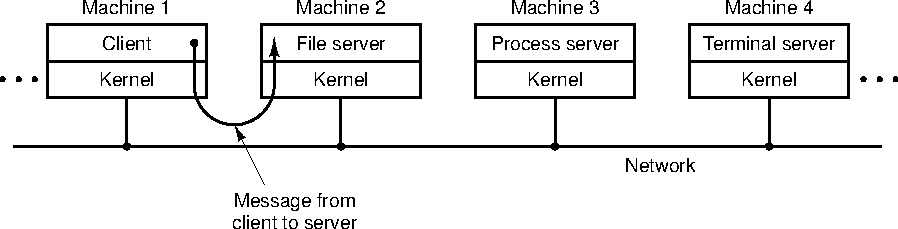
\includegraphics{fig1-27}
%   \caption{Client-Server Communication Involving the Client, a Server, and the Kernel.}
%   \label{fig:clientserver}
% \end{figure}
% 
\item ({\bf 10 Points}) It is important for the memory management unit (MMU) to be able to track the memory that is
  currently free.  Answer the following questions about managing free memory.

  \begin{enumerate}
          
  \item ({\bf 6 Points}) Suppose that the memory manager keeps a linked list of allocated and free segments.  Next,
    assume that the MMU tracks the following information for each unit of the memory; in this notation $P$
    denotes ``Process'' and $H$ stands \mbox{for ``Hole''}.

    \begin{itemize}
      \item The type marker, $T \in \{P, H\}$
      \item The start location, $S$
      \item The length of the unit, $L$
    \end{itemize}

    Using the aforementioned information that is tracked for each allocation unit, please clearly explain how the
    following memory allocation algorithms would work.

    \begin{enumerate}
      \item ({\bf 2 Points}) First fit
      \item ({\bf 2 Points}) Best fit
      \item ({\bf 2 Points}) Worst fit
      % \item ({\bf 2 Points}) Quick fit
    \end{enumerate}

  \item ({\bf 4 Points}) The memory manager should use an efficient algorithm to allocate a program to a free location in
    memory.  What is the worst-case time complexity of the first fit and best fit algorithms?  Which, if any, of these
    two algorithms is likely to be faster?

  \end{enumerate}

  \newpage

\item ({\bf 10 Points}) An operating system's memory manager often segments the memory into pages.  Answer the following
  questions about memory pages and page replacement algorithms.

  \begin{enumerate}

    \item ({\bf 2 Points}) What is a page fault? What does an operating system do when one occurs?

    \item ({\bf 2 Points}) The optimal page replacement algorithm is the ``gold standard'' by which other page
      replacement algorithms are judged.  How does this algorithm work? 
  
  \end{enumerate}

  \newpage
  
\item ({\bf 10 Points}) The process is the main ``unit of work'' in an operating system.  Answer the following questions
  about processes and how they are managed by the operating system.

  \begin{enumerate}

    \item ({\bf 4 Points}) There are four events that can lead to the creation of a process. \mbox{What are they}?

    \item ({\bf 4 Points}) A process can be in one of three states: running, blocked, and ready. Using circles to
      represent each of these states and directed edges to denote transitions between these states, draw a process-state
      diagram. All states and edges must have labels.

    \item ({\bf 2 Points}) The operating system maintains a process table that stores information about each process
      that is currently executing on a computer. Using concrete examples whenever possible, please name and describe at
      least two of these fields.

  \end{enumerate}

  \newpage

  \begin{figure}[t]
    \centering
    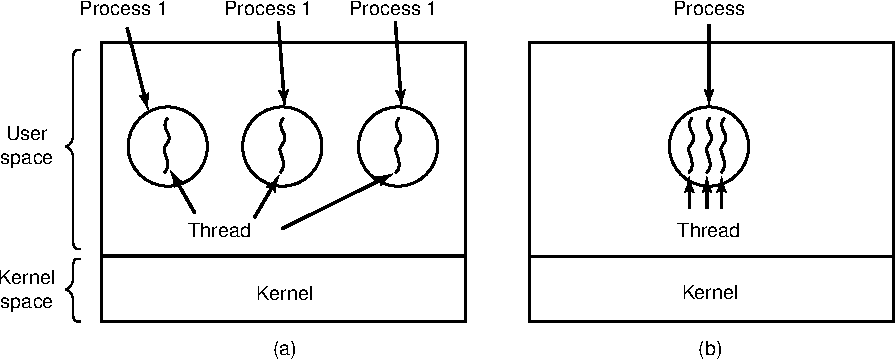
\includegraphics{fig2-11}
    \caption{Different Configurations of Processes and Threads.}
    \label{fig:pandt}
  \end{figure}


\item ({\bf 10 Points}) The operating system must provide primitives for scheduling threads and processes in a manner
  that avoids concurrency control problems. Answer the following questions about threads, processes, and concurrent
  execution.

\begin{enumerate}

  \item ({\bf 5 Points}) Figure~\ref{fig:pandt} shows two different canonical configurations of processes and threads. Answer the
    following questions about the trade-offs evident in this diagram.

    \begin{enumerate}

      \item Describe a scenario in which Figure~\ref{fig:pandt}(a) is:

        \begin{itemize}

          \item A good option for concurrent execution
          \item A poor option for concurrent execution

        \end{itemize}

      \item Describe a scenario in which Figure~\ref{fig:pandt}(b) is:

        \begin{itemize}

          \item A good option for concurrent execution
          \item A poor option for concurrent execution

        \end{itemize}

      \item If you were designing an operating system that could only support one of these models, which would you pick?
        Please justify your response to this question.

    \end{enumerate}

  \item ({\bf 5 Points}) Many kernel-mode and user-mode programs contain critical region(s) representing code
    segments that must be executed in mutual exclusion.  What is mutual exclusion? What are the four conditions that
    must be supported by any technique that aims to enforce mutual exclusion for a program's critical region?

\end{enumerate}

\end{enumerate}

\end{document}

